\documentclass[11pt]{article}
%https://www.gradescope.com/help#help-center-item-answer-formatting-guide
\usepackage{graphicx}
\usepackage{wrapfig}
\usepackage{url}
\usepackage{wrapfig}
\usepackage{color}
\usepackage{marvosym}
\usepackage{enumerate}
\usepackage{subfigure}
\usepackage{tikz}
\usepackage[fleqn]{amsmath}
\usepackage{amssymb}
\usepackage{hyperref} 
\usepackage[many]{tcolorbox}
\usepackage{lipsum}
\usepackage{float}
\usepackage{trimclip}
\usepackage{listings}
\usepackage{environ}% http://ctan.org/pkg/environ
\usepackage{wasysym}
\usepackage{array}


\oddsidemargin 0mm
\evensidemargin 5mm
\topmargin -20mm
\textheight 240mm
\textwidth 160mm

\bgroup
\def\arraystretch{1.5}
\newcolumntype{x}[1]{>{\centering\arraybackslash\hspace{0pt}}p{#1}}
\newcolumntype{z}[1]{>{\centering\arraybackslash}m{#1}}



%Arguments are 1 - height, 2 - box title
\newtcolorbox{textanswerbox}[2]{%
 width=\textwidth,colback=white,colframe=blue!30!black,floatplacement=H,height=#1,title=#2,clip lower=true,before upper={\parindent0em}}
 
 \newtcolorbox{eqanswerbox}[1]{%
 width=#1,colback=white,colframe=black,floatplacement=H,height=3em,sharp corners=all,clip lower=true,before upper={\parindent0em}}
 
 %Arguments are 1 - height, 2 - box title
 \NewEnviron{answertext}[2]{
 	\noindent
	\marginbox*{0pt 10pt}{
  	\clipbox{0pt 0pt 0pt 0pt}{
	\begin{textanswerbox}{#1}{#2}
	\BODY
	\end{textanswerbox}
	}
	}
}

%Arguments are 1 - height, 2 - box title, 3 - column definition
 \NewEnviron{answertable}[3]{
 	\noindent
	\marginbox*{0pt 10pt}{
  	\clipbox{0pt 0pt 0pt 0pt}{
	\begin{textanswerbox}{#1}{#2}
		\vspace{-0.5cm}
        		\begin{table}[H]
        		\centering 
        		\begin{tabular}{#3}
        			\BODY
        		\end{tabular}
        		\end{table}
	\end{textanswerbox}
	}
	}
}

 %Arguments are 1 - height, 2 - box title, 3 - title, 4- equation label, 5 - equation box width
 \NewEnviron{answerequation}[5]{
 	\noindent
	\marginbox*{0pt 10pt}{
  	\clipbox{0pt 0pt 0pt 0pt}{
	\begin{textanswerbox}{#1}{#2}
		\vspace{-0.5cm}
        		\begin{table}[H]
        		\centering 
		\renewcommand{\arraystretch}{0.5}% Tighter

        		\begin{tabular}{#3}
        			#4 =	&
		  	\clipbox{0pt 0pt 0pt 0pt}{

			\begin{eqanswerbox}{#5}
				$\BODY$
			\end{eqanswerbox}
			} \\ 
        		\end{tabular}
        		\end{table}
		
	\end{textanswerbox}
	}
	}
}

 %Arguments are 1 - height, 2 - box title
 \NewEnviron{answerderivation}[2]{
 	\noindent
	\marginbox*{0pt 10pt}{
  	\clipbox{0pt 0pt 0pt 0pt}{
	\begin{textanswerbox}{#1}{#2}
	\BODY
	\end{textanswerbox}
	}
	}
}

\newcommand{\vwi}{{\bf w}_i}
\newcommand{\vw}{{\bf w}}
\newcommand{\vx}{{\bf x}}
\newcommand{\vy}{{\bf y}}
\newcommand{\vxi}{{\bf x}_i}
\newcommand{\yi}{y_i}
\newcommand{\vxj}{{\bf x}_j}
\newcommand{\vxn}{{\bf x}_n}
\newcommand{\yj}{y_j}
\newcommand{\ai}{\alpha_i}
\newcommand{\aj}{\alpha_j}
\newcommand{\X}{{\bf X}}
\newcommand{\Y}{{\bf Y}}
\newcommand{\vz}{{\bf z}}
\newcommand{\msigma}{{\bf \Sigma}}
\newcommand{\vmu}{{\bf \mu}}
\newcommand{\vmuk}{{\bf \mu}_k}
\newcommand{\msigmak}{{\bf \Sigma}_k}
\newcommand{\vmuj}{{\bf \mu}_j}
\newcommand{\msigmaj}{{\bf \Sigma}_j}
\newcommand{\pij}{\pi_j}
\newcommand{\pik}{\pi_k}
\newcommand{\D}{\mathcal{D}}
\newcommand{\el}{\mathcal{L}}
\newcommand{\N}{\mathcal{N}}
\newcommand{\vxij}{{\bf x}_{ij}}
\newcommand{\vt}{{\bf t}}
\newcommand{\yh}{\hat{y}}
\newcommand{\code}[1]{{\footnotesize \tt #1}}
\newcommand{\alphai}{\alpha_i}

\newcommand{\Checked}{{\LARGE \XBox}}%
\newcommand{\Unchecked}{{\LARGE \Square}}%
\newcommand{\TextRequired}{{\textbf{Place Answer Here}}}%
\newcommand{\EquationRequired}{\textbf{Type Equation Here}}%


\newcommand{\answertextheight}{5cm}
\newcommand{\answertableheight}{4cm}
\newcommand{\answerequationheight}{2.5cm}
\newcommand{\answerderivationheight}{14cm}

\newcounter{QuestionCounter}
\newcounter{SubQuestionCounter}[QuestionCounter]
\setcounter{SubQuestionCounter}{1}

\newcommand{\subquestiontitle}{Question \theQuestionCounter.\theSubQuestionCounter~}
\newcommand{\newquestion}{\stepcounter{QuestionCounter}\setcounter{SubQuestionCounter}{1}\newpage}
\newcommand{\newsubquestion}{\stepcounter{SubQuestionCounter}}


\lstset{language=[LaTeX]TeX,basicstyle=\ttfamily\bf}

\markboth{Homework 3}{Fall 2018 CS 475 Machine Learning: Homework 3}

\title{CS 475 Machine Learning: Homework 3\\Deep Learning}
\author{Eric Rothman \\ (erothma6)} 
\date{} 



\begin{document}
\maketitle
\thispagestyle{headings}

\section*{Instructions } 
We have provided this \LaTeX{} document for turning in homework 3. We give you one or more boxes to answer each question.  The question to answer for each box will be noted in the title of the box.

 {\bf Other than your name, do not type anything outside the boxes. Leave the rest of the document unchanged.}
 
 For written answers, replace the \lstinline{\TextRequired} (\TextRequired) command with your answer. For the following example \textit{\subquestiontitle}, you would place your answer where \lstinline{\TextRequired} (\TextRequired) is located,

\begin{answertext}{1.5cm}{\subquestiontitle}
\TextRequired
\end{answertext}
\newsubquestion
 Do not change the height or title of the box. If your text goes beyond the box boundary, it will be cut off.  We have given sufficient space for each answer, so please condense your answer if it overflows. The height of the box is an upper bound on the amount of text required to answer the question - many answers can be answered in a fraction of the space.  Do not add text outside of the boxes. We will not read it.
 
For True/False or Multiple Choice questions, place your answers within the defined table.  To mark the box(es) corresponding to your answers, replace \lstinline{\Unchecked} (\Unchecked) commands with the \lstinline{\Checked} (\Checked) command. Do not make any other changes to the table. For example, in \textit{\subquestiontitle},

\begin{answertable}{2.5cm}{\subquestiontitle}{x{0.5cm}p{5cm}}
\Checked &  Logistic Regression \\ 
\Unchecked & Perceptron \\     
\end{answertable}
\newsubquestion
For answers that require a single equation, we will provide a specific type of box, such as in the following example \textit{\subquestiontitle}.  Please type the equation where  \lstinline{\EquationRequired} (\EquationRequired) without adding any \$ signs or \lstinline{\equation} commands.  Do not put any additional text in this field.

\begin{answerequation}{\answerequationheight}{\subquestiontitle}{z{1cm}z{12cm}}{\textbf{w}}{12cm}
\EquationRequired
\end{answerequation}
\newsubquestion
For answers that require multiple equations, such as a derivation, place all equations within the specified box.   You may include text short explanations if you wish (as shown in \textit{\subquestiontitle}).  You can put the equations in any format you like (e.g. within \$ or \$\$, the \lstinline{\equation} environment, the \lstinline{\align} environment) as long as they stay within the box.

\begin{answerderivation}{6cm}{\subquestiontitle}
\begin{align*}
x + 2  && \text{x is a real number} \\
&&\text{the following equation uses the variable } y \\
y+3
\end{align*}
\end{answerderivation}
\newsubquestion
\begin{center}

\textbf{Do not change any formatting in this document, or we may be unable to grade your work. This includes but is not limited to the height of textboxes, font sizes, and the spacing of text and tables.  Additionally, do not add text outside of the answer boxes. Entering your answers are the only changes allowed.}


\textbf{We strongly recommend you review your answers in the generated PDF to ensure they appear correct. We will grade what appears in the answer boxes in the submitted PDF, NOT the original latex file.}
\end{center}

% \newquestion
% \section*{\arabic{QuestionCounter}) Comparing Models  } 
% {
% \renewcommand{\answertableheight}{5cm}

% \begin{answertable}{\answertableheight}{\subquestiontitle Check All that Apply}{x{0.5cm}p{12cm}}
% \Unchecked &  Perceptron (standard) \\ 
% \Unchecked &  Logistic Regression \\ 
% \Unchecked & Support Vector Machine (with kernels) \\  
% \Unchecked & 2-Layer Feedforward Neural Network (with sigmoid activation functions) \\
% \Unchecked & None \\     
% \end{answertable}
% \newsubquestion

% \begin{answertable}{\answertableheight}{\subquestiontitle Check All that Apply}{x{0.5cm}p{12cm}}
% \Unchecked &  Perceptron (standard) \\ 
% \Unchecked &  Logistic Regression \\ 
% \Unchecked & Support Vector Machine (with kernels) \\     
% \Unchecked & 2-Layer Feedforward Neural Network (with sigmoid activation functions) \\
% \Unchecked & None \\     
% \end{answertable}
% \newsubquestion

% \begin{answertable}{\answertableheight}{\subquestiontitle Check All that Apply}{x{0.5cm}p{12cm}}
% \Unchecked &  Perceptron (standard) \\ 
% \Unchecked &  Logistic Regression \\ 
% \Unchecked & Support Vector Machine (with kernels) \\    
% \Unchecked & 2-Layer Feedforward Neural Network (with sigmoid activation functions) \\ 
% \Unchecked & None \\     
% \end{answertable}
% \newsubquestion

% \begin{answertable}{\answertableheight}{\subquestiontitle Check All that Apply}{x{0.5cm}p{12cm}}
% \Unchecked &  Perceptron (standard) \\ 
% \Unchecked &  Logistic Regression \\ 
% \Unchecked & Support Vector Machine (with kernels) \\     
% \Unchecked & 2-Layer Feedforward Neural Network (with sigmoid activation functions) \\
% \Unchecked & None \\     
% \end{answertable}
% \newsubquestion


% }

\newquestion

\section*{\arabic{QuestionCounter}) Dropout }
{
\renewcommand{\answertextheight}{8cm}

\begin{answertext}{\answertextheight}{\subquestiontitle Advantages}
The advantages of this is, much like the neural network, it decreases the dependency of the answer on a certain feature.

So in general it should decrease variance and overfitting.

Also much like in the case of neural networks, it would act as a kind of average over all the different svm's, sort of like boosting would.

It would give the same result as adding more data or adding noise to the data, which should make the trained SVM more rebust in general.

This would occur because each time an element is dropped out it makes an entire new data vector with that element 0 but every other element still what they used to be.

So in conclusion it should decrease variance.
\end{answertext}
\newsubquestion

\begin{answertext}{\answertextheight}{\subquestiontitle Disadvantages}
There are many problems with this though.

Unlike general neural networks, but still could apply to specific networks, the SVM relies on the data vector to act like a guassian to calculate max min margin.

When an elements guassian position is changed, it could drastically impact the correctness of the SVM.

So it would take longer to train to guarentee that the SVM found is the optimal one.

In addition when a feature is zeroed, it no longer becomes sure that the data the SVM is training on that round is linearly seperable.

This is especailly true in data sets with a lot of features.
zeroing an element in one of those data sets will most likely affect the linearity of the set more than actually helping remove variance.
\end{answertext}
\newsubquestion
}

\newquestion

\section*{\arabic{QuestionCounter}) Neural Networks  } 
{
\renewcommand{\answertextheight}{5cm}

\begin{answertext}{\answertextheight}{\subquestiontitle}
What might be happening is that there are hidden features and connections in the data that can't come out within one layer of linear functions through nonlinear function.

If the data was organized such that the best features to learn on are hierarchical in nature, like image processing or connections between age/physical body ratio and location for example.

That could not be captured in a single layer network.
\end{answertext}
\newsubquestion


\begin{answertext}{\answertextheight}{\subquestiontitle}
This likely occurs in the neural network because the training data was overfit on by network.

A deeper network has more parts that are fit to the data, so every parameter is being accounted for even more since it impacts several different weights.

So a deeper network is more likely to overfit without precautions being taken since every variable is more relied on, so there is more variance in the trained data when a change occurs in the test data.

Finally a deeper network will diminish the gradient of the bottom layers when using back proprogation if its too long, also causing overfitting.
\end{answertext}
\newsubquestion


\begin{answertext}{\answertextheight}{\subquestiontitle}
There are several different solutions that can be taken.

One of the most useful ones is dropout, where nodes are randomly dropped from the network during testing.

Other techniques would include adding more data, randomly augmenting data to create more data, and adding normalization to the training. 
\end{answertext}
\newsubquestion

\begin{answertext}{2cm}{\subquestiontitle}
\TextRequired
\end{answertext}
\newsubquestion
}

\newquestion

\section*{\arabic{QuestionCounter}) Backpropagation } 
{
\renewcommand{\answertableheight}{2.5cm}
\renewcommand{\answertextheight}{6cm}

\begin{answertable}{\answertableheight}{\subquestiontitle a ~Yes/No}{x{0.5cm}p{5cm}}
\Checked &  Yes \\ 
\Unchecked &  No \\ 
\end{answertable}

\begin{answertable}{\answertableheight}{\subquestiontitle b Yes/No}{x{0.5cm}p{5cm}}
\Checked &  Yes \\ 
\Unchecked &  No \\ 
\end{answertable}


\begin{answertext}{4cm}{\subquestiontitle c Loss (to 2 decimal places) or Justification}
0.04
\end{answertext}
\newsubquestion

\begin{answerequation}{\answerequationheight}{\subquestiontitle}{z{2cm}z{12cm}}{\textbf{$J(x_1,x_2)$}}{12cm}
-log(\sigma(1.1*\sigma(0.2x_1 + x_2) + 0.4*\sigma(0.3x_1 + 0.1x_2)))
\end{answerequation}
\newsubquestion

\begin{answerderivation}{\answerderivationheight}{\subquestiontitle Backpropagation partial derivative updates}
$\frac{dJ}{dy} = y*\frac{1}{y} + (1 - y*)\frac{1}{y-1}$\\
$\frac{dJ}{db} = \frac{dJ}{dy}\frac{dy}{db}, \frac{dy}{db} = \frac{e^b}{(e^b + 1)^2}$\\
$\frac{dJ}{dz_1} = \frac{dJ}{db}\frac{db}{dz_1}, \frac{db}{dz_1} = \beta_1$\\
$\frac{dJ}{dz_2} = \frac{dJ}{db}\frac{db}{dz_2}, \frac{db}{dz_2} = \beta_2$\\
$\frac{dJ}{d\beta_1} = \frac{dJ}{db}\frac{db}{d\beta_1}, \frac{db}{d\beta_1} = z_1$\\
$\frac{dJ}{d\beta_2} = \frac{dJ}{db}\frac{db}{d\beta_2}, \frac{db}{d\beta_2} = z_2$\\
$\frac{dJ}{a_1} = \frac{dJ}{dz_1}\frac{dz_1}{a_1}, \frac{dz_1}{a_1} = \frac{e^{a_1}}{(e^{a_1} + 1)^2}$\\
$\frac{dJ}{a_2} = \frac{dJ}{dz_2}\frac{dz_2}{a_2}, \frac{dz_2}{a_2} = \frac{e^{a_2}}{(e^{a_2} + 1)^2}$\\
$\frac{dJ}{\alpha_{1,1}} = \frac{dJ}{a_1}\frac{a_1}{\alpha_{1,1}}, \frac{a_1}{\alpha_{1,1}} = x_1$\\
$\frac{dJ}{\alpha_{1,2}} = \frac{dJ}{a_1}\frac{a_1}{\alpha_{1,2}}, \frac{a_1}{\alpha_{1,2}} = x_2$\\
$\frac{dJ}{\alpha_{2,1}} = \frac{dJ}{a_2}\frac{a_2}{\alpha_{2,1}}, \frac{a_2}{\alpha_{2,1}} = x_1$\\
$\frac{dJ}{\alpha_{2,2}} = \frac{dJ}{a_2}\frac{a_2}{\alpha_{2,2}}, \frac{a_2}{\alpha_{2,2}} = x_2$\\
$\frac{dJ}{x_1} = \frac{dJ}{a_1}\frac{a_1}{x_1}, \frac{a_1}{x_1} = \alpha_{1,1} + \alpha_{2,1}$\\
$\frac{dJ}{x_2} = \frac{dJ}{a_2}\frac{a_2}{x_2}, \frac{a_2}{x_2} = \alpha_{1,2} + \alpha_{2,2}$\\
$\beta$ is the weights on the linear part of the output layer and $\alpha$ are the weights on the linear parts of the hidden layer.
\end{answerderivation}

}


\newpage

\section*{Notebook Questions } 
{

\renewcommand{\answertextheight}{2cm}

\begin{answerequation}{\answerequationheight}{Question 1.5.2a}{z{9cm}z{2cm}}{Approximate accuracy for random classifier, rounded to whole integer}{2cm}
20
\end{answerequation}

\begin{answerequation}{\answerequationheight}{Question 1.5.2b}{z{9cm}z{2cm}}{Approximate accuracy for majority-vote classifier, rounded to whole integer}{2cm}
20
\end{answerequation}

\newsubquestion

\begin{answerequation}{\answerequationheight}{Question 1.5.7a}{z{4cm}z{4cm}}{Number of Weights}{4cm}
68100
\end{answerequation}

\begin{answerequation}{\answerequationheight}{Question 1.5.7b}{z{4cm}z{4cm}}{Number of Biases}{4cm}
105
\end{answerequation}

\newsubquestion

\begin{answerequation}{\answerequationheight}{Question 1.5.20a}{z{4cm}z{4cm}}{Best Validation accuracy, rounded to whole integer}{4cm}
76
\end{answerequation}

\begin{answerequation}{\answerequationheight}{Question 1.5.20b}{z{4cm}z{4cm}}{Time taken, in seconds, rounded to whole integer}{4cm}
44
\end{answerequation}

\begin{answertable}{2.5cm}{Question 1.5.20c: Did training take 10 times longer than in the case of pure SGD?}{x{0.5cm}p{5cm}}
\Unchecked &  Yes \\ 
\Checked &  No \\ 
\end{answertable}

\newsubquestion

\newsubquestion

\renewcommand{\answertextheight}{12cm}

\begin{answertext}{\answertextheight}{Question 1.5.22}
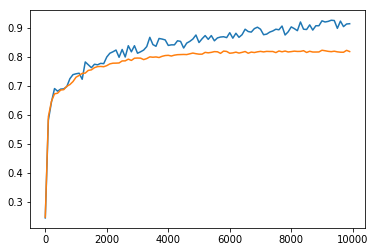
\includegraphics[height=9cm]{1_5bestpicture}
\end{answertext}



\renewcommand{\answertextheight}{6cm}
\begin{answertext}{\answertextheight}{Question 1.6.2. Compare comvolutional filters to fully connected NN}
Its different. In full neural networks, each pixel/region would be an independent input and node in the network.
In the covolution, the filters and the regions mapped through the filters are what is saved.
So the filters are like the linear function for the fully connected NN.

Instead of having to calculate the weight of each function, the convolution network can calculate the weight for each part of the a filter.
This allows for more possiblities to be stored in an easier way.
It also means that the fact that parts of images give information and group up with other parts can be preserved rather than in straing linear where they get cut off depending on the number of nodes.
\end{answertext}
\newsubquestion

\begin{answerequation}{\answerequationheight}{Question 1.6.6a}{z{9cm}z{2cm}}{Best validation accuracy, rounded to whole integer}{2cm}
76
\end{answerequation}

\begin{answerequation}{\answerequationheight}{Question 1.6.6b}{z{9cm}z{3cm}}{Time taken, in seconds, rounded to whole integer}{3cm}
25
\end{answerequation}
\newsubquestion


\begin{answerequation}{\answerequationheight}{Question 1.6.9a}{z{9cm}z{2cm}}{Best validation accuracy, rounded to whole integer}{2cm}
88
\end{answerequation}

\begin{answerequation}{\answerequationheight}{Question 1.6.9b}{z{4cm}z{3cm}}{Batch size}{3cm}
800
\end{answerequation}

\begin{answerequation}{\answerequationheight}{Question 1.6.9c}{z{4cm}z{3cm}}{Learning rate}{3cm}
0.01
\end{answerequation}

\begin{answerequation}{\answerequationheight}{Question 1.6.9d}{z{8cm}z{3cm}}{Number of optimization steps taken}{3cm}
3500
\end{answerequation}

\begin{answerequation}{\answerequationheight}{Question 1.6.9e}{z{9cm}z{3cm}}{Time taken, in seconds, rounded to whole integer}{3cm}
630
\end{answerequation}
\newsubquestion


\renewcommand{\answertextheight}{15cm}
\begin{answertext}{\answertextheight}{Question 1.7.2.8}
The starting place was my answer from 1.6.9 which I changed to have a larger validation accuracy.

I eventually settled on Adam with a learning rate of 1e-3 at the start and an SGD of a learning rate of 1e-4 for when the network's val accuracy converges past a certain point.
This is to ensure that the training settles on the local minimum.
I tried every adjustment I could, including everything from adding dropout, batch normalization, and both.
I increased the number of convolution layers and linear layers while also increasing the number of sieves/hidden nodes to be able to capture more data.
I also increased and decreased the kernel size, how many layers and which layers were pooled, whether avg or max pool should be used, the weights for the adam optimization, and I preprocessed the data by normalizing it and adding some images to the training set by vertically flipping random images in the original set.

Training was sometimes too slow when the bin size was large, like 1000.
To remedy this I decreased the bin size so that less examples were trained on at once.
I also tried to pool as soon as possible so that the training would run faster.
The most important change I made was to either add dropout to the model or to increase the initial kernel size to 5 or to add pooling earlier on in the training with a kernel of size 3.

I have 2 different models. I will talk about the one that did the best which is the 2nd one, and the one my optimal answer should have come from but for some reason I can't replicate.
This model receives an input of a 26x26 pixel image.
It then runs it through a convolution layer of kernel size 5, decreasing the new collection of features to be 22x22 with 8 sieves.
It then runs that through another convolution layer and avg pools the outcome to be an image of 6x6 and 64 sieves.
Then it runs through another layer creating the pool to be 4x4 and a final pool making it 3x3 with the first layer making the total number of sieves to be 128 and the second making it 512.
Then it pools the remaining pixels together using a max pool so that the colection is a 1x1 group.
Then it runs it through 3 linear functions with the first layer making it go from 1024 nodes to 400 and the second going from 400 hidden nodes to 200.
Finally the last layer converts the 200 hidden nodes to 5 which predict the class the image is of.
\end{answertext}
\newsubquestion


\renewcommand{\answertextheight}{6cm}

\begin{answertable}{2.5cm}{Question 1.8.4a: Are there any qualitative differences between these sets of images}{x{0.5cm}p{5cm}}
\Checked &  Yes \\ 
\Unchecked &  No \\ 
\end{answertable}

\begin{answertable}{2.5cm}{Question 1.8.4b: Are the misclassified examples more difficult for you to classify}{x{0.5cm}p{5cm}}
\Checked &  Yes \\ 
\Unchecked &  No \\ 
\end{answertable}

\renewcommand{\answertextheight}{12cm}

\begin{answertext}{\answertextheight}{Question 1.8.6}
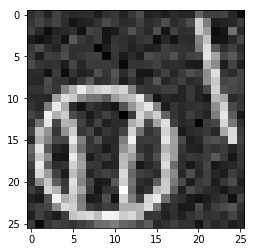
\includegraphics[height=9cm]{1_8_6_HW3}
\end{answertext}

\newsubquestion



\begin{answertable}{2.5cm}{Question 1.8.7: Does the classifier still classify all 10 images correctly}{x{0.5cm}p{5cm}}
\Checked &  Yes \\ 
\Unchecked &  No \\ 
\end{answertable}

\newsubquestion



\begin{answertable}{2.5cm}{Question 1.8.10: Does the classifier still classify all 10 images correctly}{x{0.5cm}p{5cm}}
\Checked &  Yes \\ 
\Unchecked &  No \\ 
\end{answertable}

\newsubquestion



\renewcommand{\answertextheight}{15cm}
\begin{answertext}{\answertextheight}{Question 1.8.11}
It is not necessarily a failure, for example if the image trying to be processed is text. Then when flipped horizontally, the outcome should be indecipherable gibberish or even unreadable.

There are things, like letters and numbers, which become meaning less when flipped horizontally.

For these classes though, each one has meaning when flipped horizontally, so it would be considered a failure.

To train to accomidate for the flipped images we could randomly flip images in the training set or during training time have a drop out effect sort of where instead of nodes disappearing, there is a random chance for each image in the minibatch that it will be flipped.

So during training have a line like: with p=0.1 an image will be flipped horizontally.

Exactly how often you should flip will change and is something the user should decide.

Or you could just add the flipped images to the data set as a whole at the beginning before devying up training and val data.

You could also add more nodes or use convolution layers to try to catch general patterns, not necessarily strict pixel ordering, but that might not necessarily work since you can't exactly decide what features to train on.

Out of the two things I suggested, I think convolution layers are the better choice since they are build to reuse patterns efficiently. 
\end{answertext}
\newsubquestion


}

\end{document}
